\documentclass[11pt,a4paper]{article}

% Packages
\usepackage[utf8]{inputenc}
\usepackage[T1]{fontenc}
\usepackage[margin=1in]{geometry}
\usepackage{titlesec}
\usepackage{enumitem}
\usepackage{hyperref}
\usepackage{booktabs}
\usepackage{array}
\usepackage{longtable}
\usepackage{parskip}
\usepackage{listings}
\usepackage{float}
\usepackage{svg}
\usepackage{longtable}

\usepackage{enumitem}
\usepackage{booktabs}
\usepackage{graphicx}
\usepackage{hyperref}
\usepackage{xcolor}
\usepackage{caption}
\usepackage{subcaption}
\usepackage{float}

\usepackage{forest}
\usepackage{fancyhdr}
\usepackage{tikz}
\usetikzlibrary{arrows.meta, positioning, fit, backgrounds, calc}

\hypersetup{colorlinks=true, linkcolor=blue, urlcolor=blue}
\setlength{\parindent}{0pt}
\setlength{\parskip}{6pt}

\graphicspath{{./component/figures/}}


% Page geometry
\geometry{margin=1in}

% Hyperlink setup
\hypersetup{
    colorlinks=true,
    linkcolor=blue,
    urlcolor=blue,
    citecolor=blue
}

% Title formatting
\titleformat{\section}{\large\bfseries}{\thesection}{1em}{}
\titleformat{\subsection}{\normalsize\bfseries}{\thesubsection}{1em}{}

% Document info
\title{CSC490 Assignment A3 - Pre-training Nanochat}
\author{
    Chris Jiang (Student ID: 1008109574) |
    Yihe Li (Student ID: 1009802331) \\
    Qianwen Wang (Student ID: 1009985358) |
    Seonghyun Ban  (Student ID: 1005127738)
}
\date{\today}

\begin{document}

\maketitle

We include a supplementary appendix (Appendix~\ref{sec:appendix-pipeline}) explaining our infrastructure choices and how the training pipeline works at a high level. We recommend reading it before looking into the codebase.

% Part 1: Interest Statements
\input{component/part1}

% Part 2: Landscape Analysis
\input{component/part2}

% Part 3: Project Outline

%% ============================================================
\section{Part 3: Context Window Extension}
%% ============================================================

\subsection{Overview and Findings}

Context window extension trains a language model at a short sequence length, then resumes training at a longer sequence length. The hypothesis is that most language knowledge is learned during the short-context phase, and extension mainly teaches the model to attend over longer positions---making it a cheaper alternative to training at full context from the start.

This is well-established in the literature. GrowLength~\cite{growlength} demonstrates progressive context growth (e.g.\ 128$\to$256$\to$512$\to$1024) during pretraining, finding that short-context phases contribute the bulk of capability and that extension mainly adapts attention patterns to longer positions~\cite{skyladder,prolong}.

We train ``picochat''---a smaller nanochat configuration---at sequence length 512, extend to 2048, and compare against training at 2048 from scratch. Our key findings:

\begin{itemize}
  \item Context extension mechanically works: the extended model handles long positions better than the short-only model (mean CE 4.19 vs 4.34 beyond position 512).
  \item The degradation beyond the training boundary is gradual ($+0.35$~nats), not catastrophic---RoPE extrapolation at 4$\times$ is within tolerance at this model scale.
  \item The cheap path (extension) nearly matches the expensive path (full training) on BPB (1.0540 vs 1.0499) and CORE (0.0766 vs 0.0789), but leaves a 28\% gap on PG19 perplexity (73.55 vs 57.40) due to unmitigated forgetting.
\end{itemize}

%% ============================================================
\subsection{Method and Justification}
%% ============================================================

\subsubsection{Model Configuration}

Picochat uses nanochat's depth-6 configuration:

\begin{table}[H]
\centering\small
\begin{tabular}{@{}ll@{}}
\toprule
Parameter & Value \\
\midrule
Depth & 6 \\
Model dim & 384 \\
Attention heads & 3 \\
Head dim & 128 \\
Window pattern & SSSL \\
Total parameters & ${\sim}136$M \\
Scaling parameters & ${\sim}35.8$M \\
\bottomrule
\end{tabular}
\end{table}

Depth~6 is the smallest nanochat configuration with 3 attention heads (depth~4 has only 2). Nanochat's own \texttt{runcpu.sh} uses depth~6 for demos.

\subsubsection{Sequence Length}

The target of 2048 is nanochat's default \texttt{max\_seq\_len} and the assignment requirement. No RoPE interpolation is needed---we are returning to the native context length. The question is what short length to start from.

We chose 512, grounding the decision in two sources:

\begin{enumerate}
  \item \textbf{BabyLM}~\cite{babyslen} tests 125M-parameter models across \{64, 128, 256, 512, 1024, 2048, 4096, 8192\} and recommends 512 as ``a safe and efficient baseline across both architectures.''
  \item \textbf{GrowLength}~\cite{growlength} validates 2$\times$ per-stage jumps as the established baseline for progressive context growth.
\end{enumerate}

This places our 4$\times$ jump (512$\to$2048) as a deliberate sweet spot. A 2$\times$ jump (1024$\to$2048) is already validated by GrowLength as their baseline---repeating it adds no new insight---and offers only modest compute savings since attention is a small fraction of total FLOPs at this model scale. An 8$\times$ jump (256$\to$2048) pushes further into territory that GrowLength warns against: they find that ``substantial difference between consecutive training window sizes can lead to dramatic loss rising,'' though their experiments are on multi-stage schedules, not single-stage jumps. Our 4$\times$ is a moderate extrapolation beyond the validated 2$\times$---large enough for meaningful savings, small enough to stay closer to the safe range.

\subsubsection{Data Portion}

The token budget of ${\sim}376$M is 0.38\% of the FineWeb-edu 100B-token corpus. This is the compute-optimal amount for a 35.8M scaling-parameter model under nanochat's 10.5$\times$ data ratio, which follows Chinchilla-style scaling laws~\cite{chinchilla}. We use nanochat's default ratio because the codebase's hyperparameters (LR, batch size, weight decay) are co-tuned for it.

This gives a three-stage experiment:

\begin{table}[H]
\centering\small
\begin{tabular}{@{}lllrl@{}}
\toprule
Stage & Strategy & seq\_len & Steps & Purpose \\
\midrule
1 & Train from scratch & 512 & 1433 & Short-context pretraining \\
2 & Resume from Stage~1 & 2048 & 500 (1433$\to$1933) & Context extension (cheap path) \\
3 & Train from scratch & 2048 & 1433 & Full-context baseline (expensive path) \\
\bottomrule
\end{tabular}
\end{table}

Stages~1 and~3 use nanochat's auto-computed iteration count (\texttt{target\_tokens / total\_batch\_size} $= 375{,}732{,}000 / 262{,}144 \approx 1433$). The literature provides no quantitative recovery data for single-stage context jumps, so Stage~2 uses a generous 500 extension steps with \texttt{save\_every=50} to observe the actual trajectory at high resolution (10 intermediate checkpoints). In hindsight, recovery largely plateaus by step~${\sim}1600$ (${\sim}170$ steps in), so fewer steps would have sufficed---but this was unknown beforehand. On resume, nanochat recalculates the LR schedule for \texttt{num\_iterations=1933}, producing a deliberate rewarm from ${\approx}0$ to ${\approx}0.52$ of peak LR at step~1433---analogous to ProLong's approach~\cite{prolong}.

\subsubsection{Custom Evaluation}

We designed a per-position cross-entropy evaluation to directly measure whether the model handles positions beyond its training length:

\begin{itemize}
  \item \textbf{Dataset}: PG19 test split---avoids contamination (nanochat trains on FineWeb-edu) and is standard in context extension literature~\cite{pi,yarn,longrope}.
  \item \textbf{Bucketing}: 128-token windows (16 buckets for 2048 tokens). Each bucket reports mean cross-entropy across all documents.
  \item \textbf{Sample}: All 100 documents in PG19 test split, each truncated to 2048 tokens.
\end{itemize}

We also run nanochat's built-in evaluations:
\begin{itemize}
  \item \textbf{BPB} (bits per byte): Overall language modeling quality on FineWeb-edu validation.
  \item \textbf{CORE} (22 tasks): General task capability. At ${\sim}136$M params, most tasks are near random---HellaSwag, PIQA, ARC-Easy, and BoolQ are the most informative. The appendix lists all 22 per-task scores.
\end{itemize}

\subsubsection{Checkpoints}

\begin{table}[H]
\centering\small
\begin{tabular}{@{}llrl@{}}
\toprule
Checkpoint & Model Tag & Step & Description \\
\midrule
Short & pico-short & 1433 & End of Stage~1 (seq\_len=512 only) \\
Extended & pico-short & 1933 & End of Stage~2 (512$\to$2048 extension) \\
Full & pico-full & 1433 & End of Stage~3 (2048 from scratch) \\
\bottomrule
\end{tabular}
\end{table}

Additionally, 10 intermediate checkpoints during extension (steps 1450--1900, every 50 steps) were evaluated with both custom eval and CORE to track recovery dynamics.

CORE was not run on the short checkpoint (pico-short@1433) because nanochat's RoPE positional encoding at seq\_len=512 cannot process the 2048-token CORE prompts.

\subsubsection{Compute Specification}

All training and evaluation ran on A100-80GB GPUs via Modal. We chose this GPU for two reasons. First, the full batch at \texttt{seq\_len=2048} (${\sim}262{,}144$ tokens) fits in 80\,GB, allowing one forward pass per optimizer step with no gradient accumulation. Second, nanochat's built-in CORE evaluation at 2048-token prompts exceeded 40\,GB VRAM, ruling out the A100-40GB. All stages use nanochat's default learning rate schedule (warmup ratio 0, warmdown ratio 0.5).



%% ============================================================
\subsection{Results}
%% ============================================================

\subsubsection{Per-Position Cross-Entropy}

\begin{figure}[H]
\centering
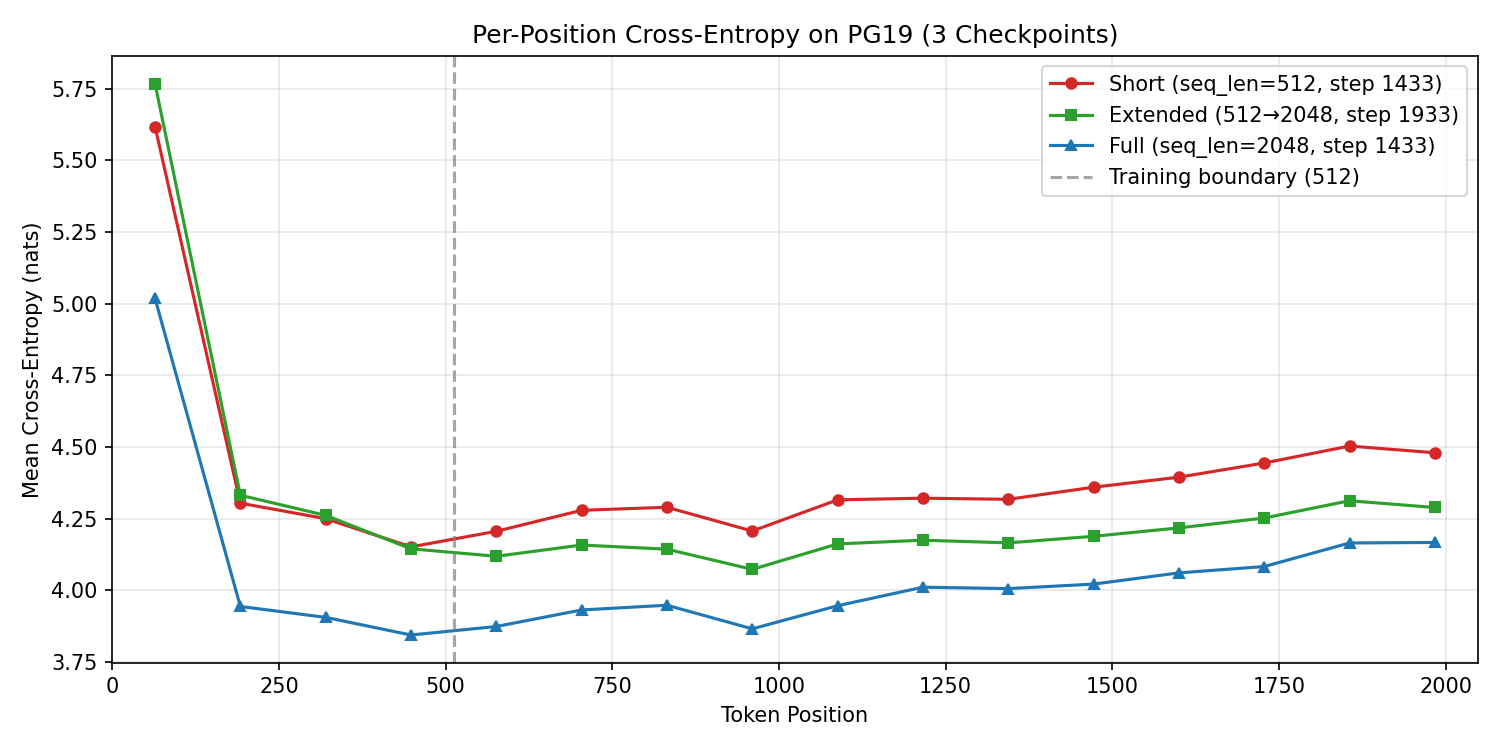
\includegraphics[width=\linewidth]{p3/per_position_ce.png}
\caption{Per-position cross-entropy on PG19 for three checkpoints. Dashed vertical line marks the 512-token training boundary.}
\label{fig:perpos}
\end{figure}

The short checkpoint (red) shows a gradual upward drift in cross-entropy beyond position~512, rising from ${\sim}4.15$ at positions 384--512 to ${\sim}4.50$ at positions 1920--2048---a $+0.35$~nats degradation. This is not catastrophic but is consistent: positions the model never trained on are handled worse.

The extended checkpoint (green) improves over short beyond position~512 (mean CE 4.19 vs 4.34, a 0.15~nats improvement), confirming that context extension mechanically worked.

The full checkpoint (blue) achieves the lowest CE at all positions, with a consistent advantage that narrows from ${\sim}0.30$--$0.40$~nats at early positions to ${\sim}0.15$~nats toward the end of the context---including positions 0--512 where both models had training data.

\subsubsection{Recovery Evolution}

\begin{figure}[H]
\centering
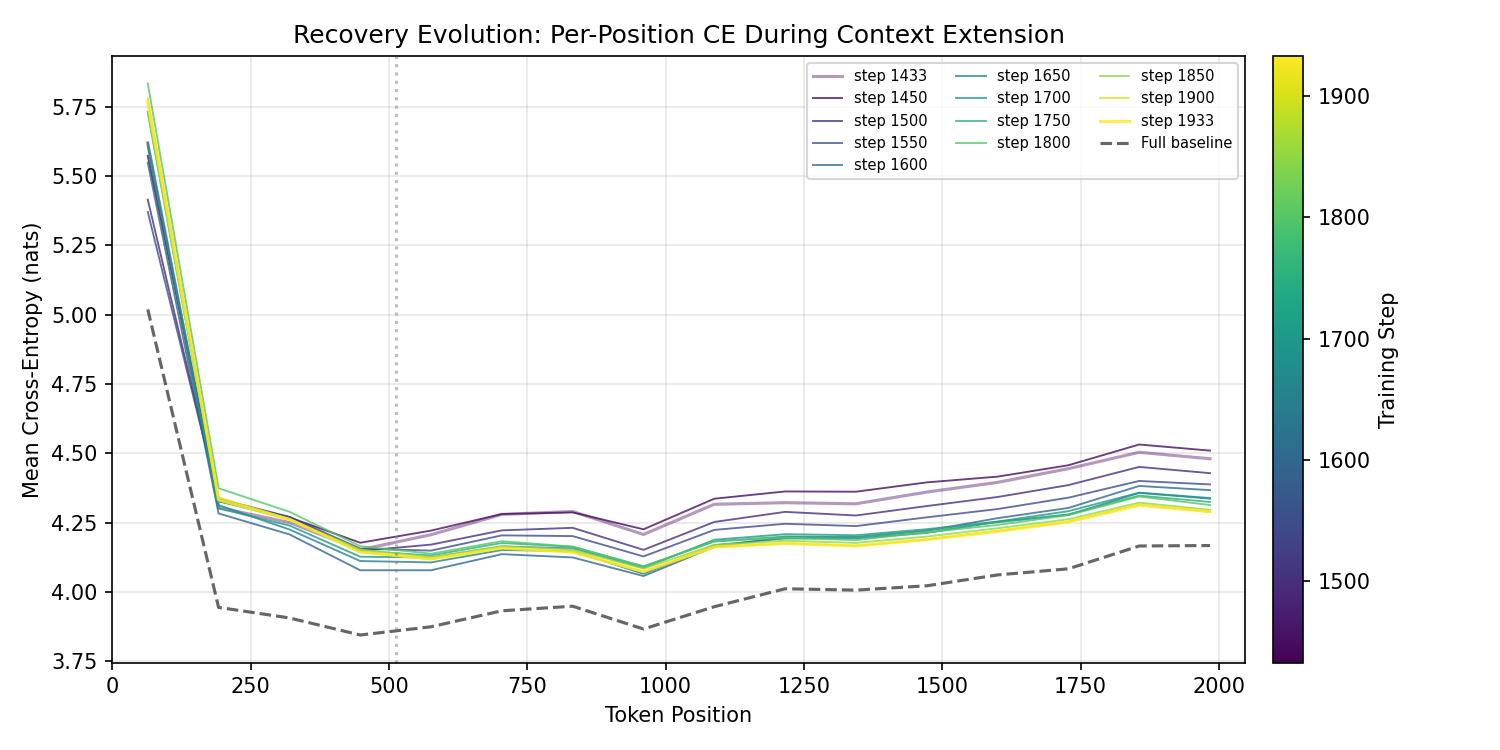
\includegraphics[width=\linewidth]{p3/recovery_evolution.png}
\caption{Per-position cross-entropy at each extension checkpoint (steps 1433--1933). Dashed black line is the full-from-scratch baseline.}
\label{fig:recovery}
\end{figure}

The model improves most rapidly in the first ${\sim}150$ extension steps (1433$\to$1600). Beyond step~1600, PG19 CE plateaus and oscillates mildly, with the final value (4.298) close to the step-1600 minimum (4.288). The largest gains are at positions 512--1024, where the model transitions from untrained to trained positions.

\subsubsection{Training Curves}

\begin{figure}[H]
\centering
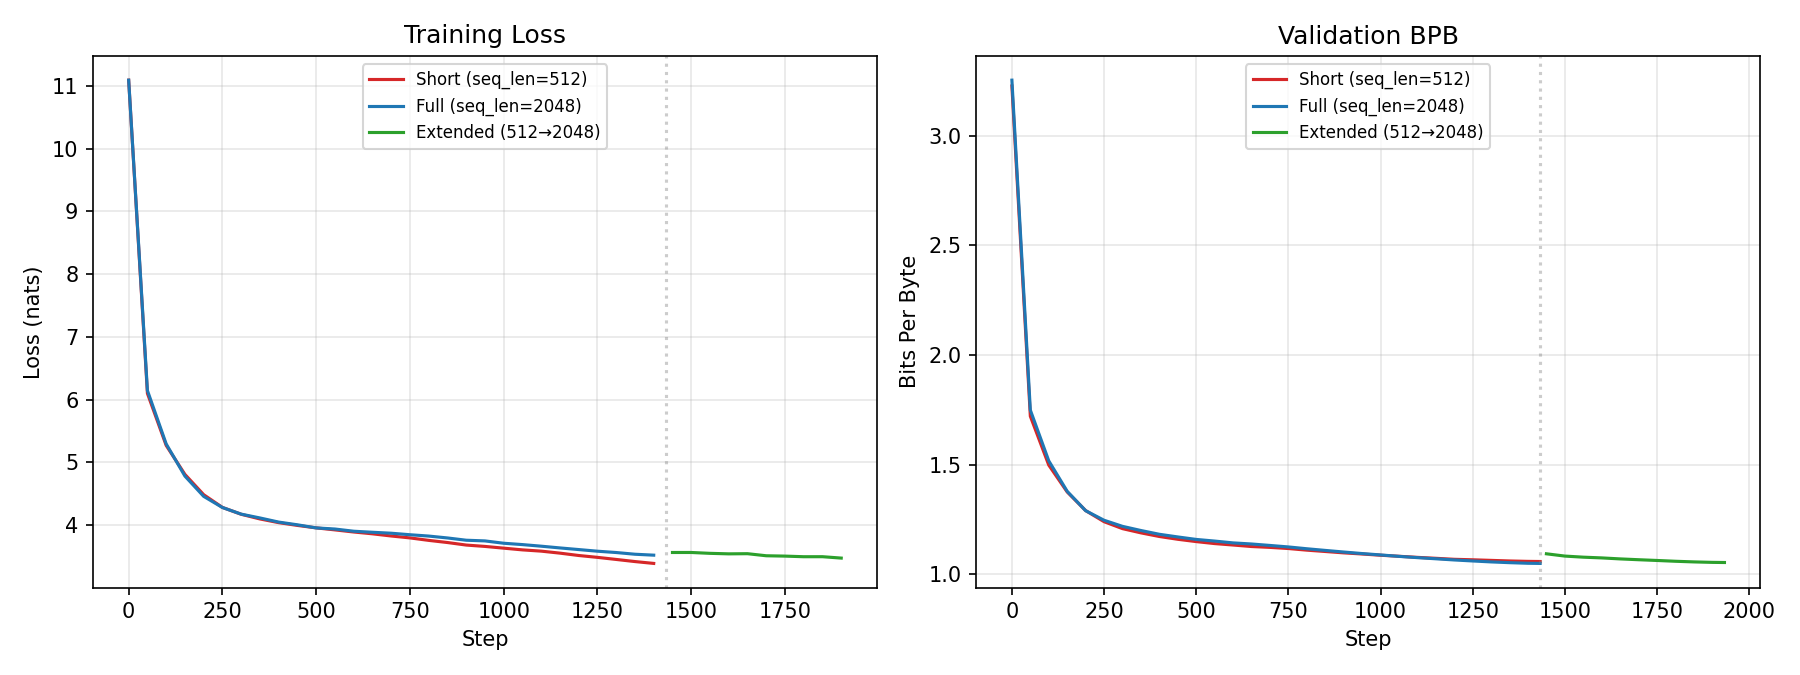
\includegraphics[width=\linewidth]{p3/training_curves.png}
\caption{Training loss (left) and validation BPB (right) from W\&B. Dotted vertical line marks step~1433 where extension begins.}
\label{fig:traincurves}
\end{figure}

Short and full training curves overlap closely---both reach similar loss levels despite different sequence lengths. The extension phase (green, steps 1433--1933) shows a mild increase in training loss at resume (from the 4$\times$ context jump and LR rewarm), followed by steady recovery. Validation BPB during extension decreases monotonically toward the full baseline.

\subsubsection{BPB and CORE Recovery}

\begin{figure}[H]
\centering
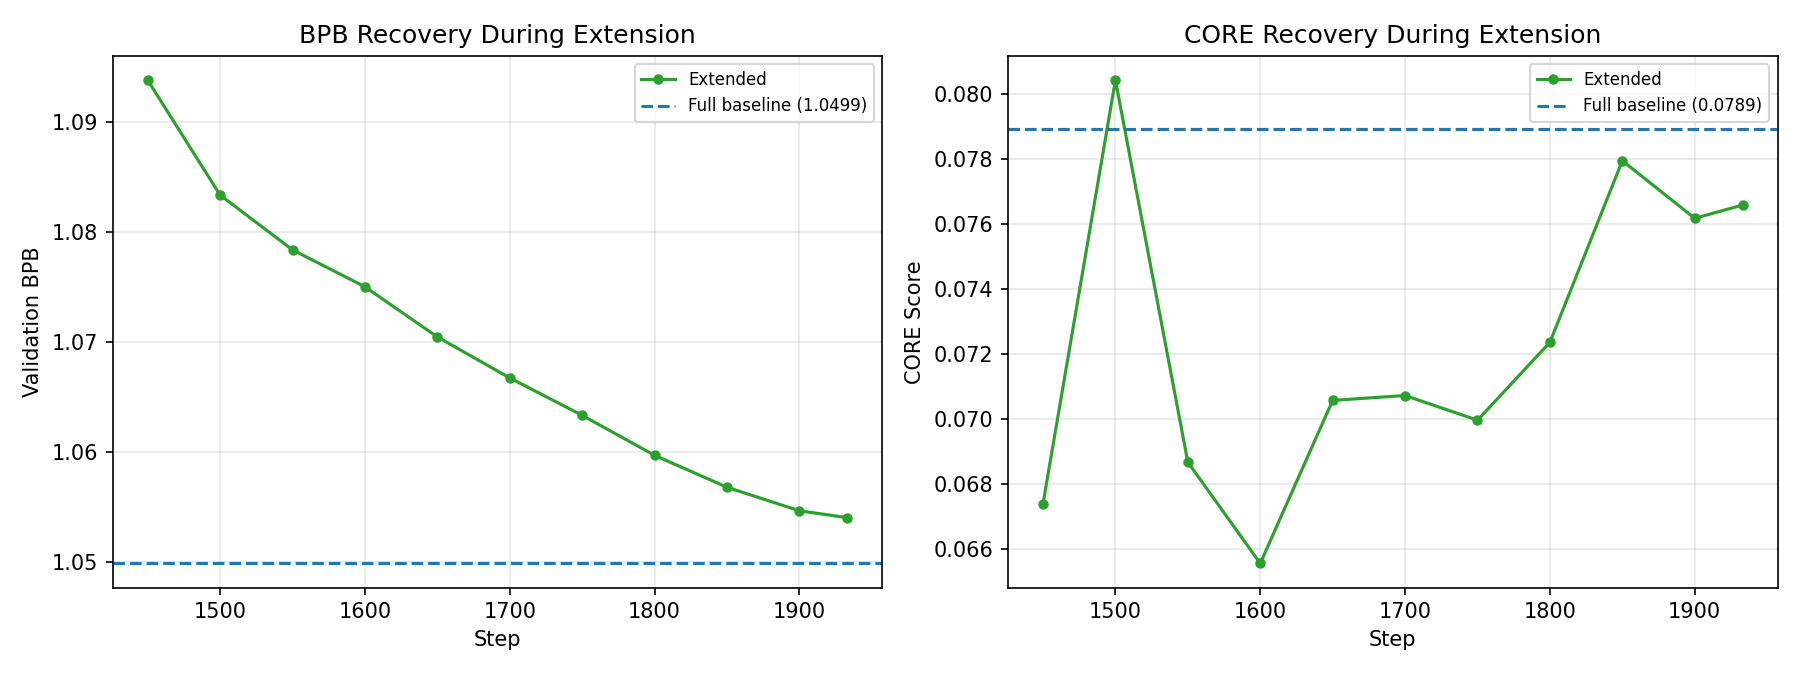
\includegraphics[width=\linewidth]{p3/bpb_core_recovery.png}
\caption{Validation BPB (left) and CORE score (right) during extension. Dashed blue line is the full-from-scratch baseline.}
\label{fig:bpbcore}
\end{figure}

BPB recovery is smooth and monotonic, approaching the full baseline (1.0540 vs 1.0499 at convergence). CORE recovery is noisier---expected at this model scale where individual task scores fluctuate---but trends upward, reaching 0.0766 vs the full baseline's 0.0789.

\subsubsection{Summary}

\begin{table}[H]
\centering\small
\begin{tabular}{@{}lccc@{}}
\toprule
Metric & Short (1433) & Extended (1933) & Full (1433) \\
\midrule
Val BPB & 1.0586 & 1.0540 & 1.0499 \\
Train Loss & 3.3921 & 3.4769 & 3.5236 \\
PG19 Aggregate CE & 4.4029 & 4.2980 & 4.0500 \\
PG19 Aggregate PPL & 81.69 & 73.55 & 57.40 \\
CE (pos 0--512) & 4.5811 & 4.6267 & 4.1785 \\
CE (pos 512--2048) & 4.3435 & 4.1884 & 4.0071 \\
CORE & N/A & 0.0766 & 0.0789 \\
\bottomrule
\end{tabular}
\caption{Summary of all metrics. Short CORE is N/A because RoPE at seq\_len=512 cannot process 2048-token CORE prompts.}
\label{tab:summary}
\end{table}

\subsubsection{Cost Report}

\begin{table}[H]
\centering\small
\begin{tabular}{@{}lrl@{}}
\toprule
Run & GPU-Hours & Description \\
\midrule
Pipeline (baseline) & ${\sim}1.51$ & 3 stages + 3 evals \\
Pipeline (CORE recovery) & ${\sim}1.34$ & 10 CORE evals at intermediate steps \\
Debug / failed attempts & ${\sim}1.83$ & 13 smaller runs \\
\midrule
\textbf{Total} & \textbf{4.67} & \textbf{15 Modal app runs} \\
\bottomrule
\end{tabular}
\caption{GPU-hours breakdown. Estimated cost: \$29.77 at A100-80GB rates (\$6.37/hr).}
\label{tab:cost}
\end{table}

The two successful pipeline runs used ${\sim}2.85$ GPU-hours total. Debug runs account for 39\% of total cost---expected for a first-time pipeline with multiple failure modes (OOM on A100-40GB, RoPE overflow for short-context CORE, nanochat import paths, BFloat16 autocast).



%% ============================================================
\subsection{Discussion}
%% ============================================================

Context extension mechanically works: the model recovers from the 4$\times$ context jump within ${\sim}150$ steps, with BPB and CORE approaching the full-from-scratch baseline. However, a persistent PG19 perplexity gap (28\%) at all positions---including those seen during short training---indicates forgetting that nanochat's pipeline cannot mitigate. Extension is a viable cheap path for general capability but not for long-context quality.

\subsubsection{Recovery Dynamics}

On resume at step~1433, the model experiences two simultaneous shocks: a 4$\times$ context length jump (512$\to$2048) and a learning rate rewarm (from ${\approx}0$ to ${\approx}0.52$ of peak). The training loss spikes mildly (Figure~\ref{fig:traincurves}), then recovers steadily.

The recovery is front-loaded. Per-position cross-entropy improves most rapidly in the first ${\sim}150$ steps (1433$\to$1600), with the largest gains at positions 512--1024 where the model encounters truly novel positions for the first time (Figure~\ref{fig:recovery}). BPB recovery is smooth and monotonic throughout (Figure~\ref{fig:bpbcore}, left). CORE recovery is noisier but trends upward (Figure~\ref{fig:bpbcore}, right)---the noise is expected at this model scale, where individual task scores fluctuate between checkpoints.

\subsubsection{Does the Cheap Path Work?}

The cheap path (512$\to$2048 extension) nearly matches the expensive path (2048 from scratch) on general-purpose metrics:

\begin{itemize}
  \item \textbf{BPB}: 1.0540 vs 1.0499---a 0.0042 gap. Close enough for practical purposes.
  \item \textbf{CORE}: 0.0766 vs 0.0789---within noise at this model scale.
\end{itemize}

However, on the positional perplexity evaluation designed specifically for context extension, the gap is substantial: PG19 perplexity of 73.55 vs 57.40 (28\%). This gap persists at \emph{all} positions, including 0--512 where both models had training data (CE 4.63 vs 4.18). Indeed, the extended model is slightly worse than the short-only model at positions 0--512 (CE 4.63 vs 4.58), confirming that extension actively degrades performance at originally trained positions. ProLong~\cite{prolong} identifies this as forgetting: without short-context data mixing during extension, the model partially unlearns what it knew. Nanochat does not support data mixing, so this forgetting is unmitigated.

\subsubsection{Compute Efficiency}

Stage~2 ran 500 steps at seq\_len=2048 vs Stage~3's 1433 steps---roughly 65\% fewer long-context training steps. However, including the short-context phase, the progressive path uses more total compute (127.9T vs 94.8T FLOPs). The savings materialize only when extending a pre-existing short-context model, not when both paths start from scratch. Whether the trade-off is worthwhile depends on the use case: for BPB and CORE (general capability), the cheap path is viable; for tasks requiring strong long-context performance, training from scratch is preferable.

\medskip
\textbf{Limitations.}
We tested a single model scale (${\sim}136$M parameters), a single jump ratio (4$\times$), and evaluated on a single long-document dataset (PG19). ProLong's 40\% short-context data mixing---which would likely close the PG19 gap---is unavailable in nanochat. Results may differ at larger scales, with progressive multi-stage schedules (as in GrowLength), or on other evaluation domains.

%% ============================================================


\subsection*{Appendix}

\subsubsection*{W\&B Runs}

\begin{itemize}
  \item \textbf{p3-baseline-short}: \url{https://wandb.ai/seonghyun-ban-uoft/490-autobook-a3/runs/mpaiemt0}
  \item \textbf{p3-baseline-extended}: \url{https://wandb.ai/seonghyun-ban-uoft/490-autobook-a3/runs/woxwtud7}
  \item \textbf{p3-baseline-full}: \url{https://wandb.ai/seonghyun-ban-uoft/490-autobook-a3/runs/wy8sw0zf}
\end{itemize}

\subsubsection*{CORE Per-Task Breakdown for Extended Picochat and Full Picochat}
%% ============================================================

\begin{table}[H]
\centering\small
\begin{tabular}{@{}lcc@{}}
\toprule
Task & Extended (1933) & Full (1433) \\
\midrule
\textbf{CORE (aggregate)} & \textbf{0.0766} & \textbf{0.0789} \\
\midrule
hellaswag & 0.2731 & 0.2745 \\
hellaswag\_zeroshot & 0.2810 & 0.2767 \\
arc\_easy & 0.4289 & 0.4314 \\
copa & 0.6100 & 0.5500 \\
piqa & 0.5871 & 0.5996 \\
boolq & 0.4529 & 0.5899 \\
winograd & 0.5311 & 0.5018 \\
winogrande & 0.5170 & 0.5043 \\
commonsense\_qa & 0.2703 & 0.2817 \\
openbook\_qa & 0.2740 & 0.2540 \\
lambada\_openai & 0.1820 & 0.1814 \\
bigbench\_qa\_wikidata & 0.1469 & 0.1284 \\
bigbench\_cs\_algorithms & 0.3977 & 0.3886 \\
bigbench\_dyck\_languages & 0.1210 & 0.0530 \\
agi\_eval\_lsat\_ar & 0.2826 & 0.2435 \\
arc\_challenge & 0.2304 & 0.2457 \\
bigbench\_language\_id & 0.2574 & 0.2526 \\
bigbench\_operators & 0.0667 & 0.0667 \\
squad & 0.0035 & 0.0033 \\
coqa & 0.0256 & 0.0370 \\
jeopardy & 0.0005 & 0.0019 \\
bigbench\_repeat\_copy & 0.0000 & 0.0000 \\
\bottomrule
\end{tabular}
\caption{CORE per-task accuracy. Most scores are within noise. The largest differences (boolq, copa) go in opposite directions, consistent with variance rather than systematic capability gaps.}
\label{tab:core}
\end{table}

\newpage
\subsection*{References for Part 3}
\begin{thebibliography}{8}

\bibitem{growlength}
H.~Jin, X.~Han, J.~Yang, Z.~Jiang, C.-Y.~Chang, and X.~Hu.
\newblock GrowLength: Accelerating LLMs Pretraining by Progressively Growing Training Length.
\newblock \textit{arXiv:2310.00576}, 2023.

\bibitem{skyladder}
T.~Zhu, Q.~Liu, H.~Wang, S.~Chen, X.~Gu, T.~Pang, and M.-Y.~Kan.
\newblock SkyLadder: Better and Faster Pretraining via Context Window Scheduling.
\newblock \textit{NeurIPS}, 2025. arXiv:2503.15450.

\bibitem{prolong}
T.~Gao, A.~Wettig, H.~Yen, and D.~Chen.
\newblock How to Train Long-Context Language Models (Effectively).
\newblock \textit{ACL}, 2025. arXiv:2410.02660.

\bibitem{babyslen}
S.~Salhan, R.~Diehl~Martinez, Z.~Goriely, and P.~Buttery.
\newblock What is the Best Sequence Length for BabyLM?
\newblock \textit{BabyLM Workshop @ EMNLP}, 2025. arXiv:2510.19493.

\bibitem{chinchilla}
J.~Hoffmann, S.~Borgeaud, A.~Mensch, et~al.
\newblock Training Compute-Optimal Large Language Models.
\newblock \textit{NeurIPS}, 2022. arXiv:2203.15556.

\bibitem{pi}
S.~Chen, S.~Wong, L.~Chen, and Y.~Tian.
\newblock Extending Context Window of Large Language Models via Positional Interpolation.
\newblock \textit{arXiv:2306.15595}, 2023.

\bibitem{yarn}
B.~Peng, J.~Quesnelle, H.~Fan, and E.~Shippole.
\newblock YaRN: Efficient Context Window Extension of Large Language Models.
\newblock \textit{ICLR}, 2024. arXiv:2309.00071.

\bibitem{longrope}
Y.~Ding, L.~Zhang, C.~Jia, et~al.
\newblock LongRoPE: Extending LLM Context Window Beyond 2 Million Tokens.
\newblock \textit{arXiv:2402.13753}, 2024.

\end{thebibliography}




% Part 4: Press Release
\section{Part 4: Training the Final Nanochat Model}

\subsection{Motivation}

The picochat ablation experiments in Part~2 compared several architectural
modifications, including SwiGLU and LayerScale. Although the baseline
architecture achieved the best results at the pico scale, architectural
changes often behave differently as model capacity increases.

Recent large language models such as PaLM and LLaMA adopt gated MLP
variants (e.g., SwiGLU), suggesting that such modifications may become
beneficial at larger scales. Therefore, in addition to the baseline
configuration, we trained a larger nanochat model incorporating SwiGLU
to examine whether its advantages emerge under increased model capacity.

\subsection{Model Configuration}

The final nanochat models were trained using the configuration shown in
Table~\ref{tab:nano_config}. Compared to picochat, the nanochat model
increases network depth and effective batch size, enabling training on
a substantially larger token budget.

\begin{table}[H]
\centering
\begin{tabular}{lc}
\hline
\textbf{Parameter} & \textbf{Value} \\
\hline
Model Depth & 20 layers \\
Sequence Length & 512 \\
Training Iterations & 4357 \\
Device Batch Size & 32 \\
Total Batch Size & 1,048,576 \\
GPU Type & H100 \\
Precision & FP8 (tensorwise) \\
Window Pattern & L \\
\hline
\end{tabular}
\caption{Nanochat training configuration.}
\label{tab:nano_config}
\end{table}

Training was performed on the full pretraining dataset using
the nanochat training framework.

Two models were trained:

\begin{itemize}
\item \textbf{Nanochat Baseline}: standard ReLU$^2$ MLP.
\item \textbf{Nanochat SwiGLU}: identical architecture with a SwiGLU MLP block.
\end{itemize}

\subsection{Training Procedure}

Training was conducted on H100 GPUs via Modal using FP8 tensorwise
precision to improve throughput and memory efficiency. Training progress
was monitored using Weights \& Biases.

Both models exhibited nearly identical loss trajectories throughout
training, indicating similar optimization behavior. However, the SwiGLU
model showed lower token throughput due to the additional gating
operations within the MLP block.

\subsection{Scaling Prediction}

Before training the nanochat models, we estimate how performance should
change when scaling from picochat (6 layers) to nanochat (20 layers).

The picochat baseline achieved:

\begin{itemize}
\item BPB: 1.0575
\item CORE: 0.0615
\end{itemize}

Increasing model capacity and training compute should significantly
improve language modeling performance. We therefore predict that the
nanochat model will achieve substantially lower BPB and higher CORE
scores than picochat.

After training, the results confirm this prediction. The nanochat
baseline achieves:

\begin{itemize}
\item Validation BPB: 0.7822
\item CORE score: 0.2038
\end{itemize}

This corresponds to roughly a \textbf{26\% reduction in BPB} and more
than a \textbf{threefold increase in CORE}. The improvement is far larger
than the differences between architectural variants, indicating that
model scale is the dominant factor affecting performance.

\subsection{Evaluation}

Following the evaluation protocol in the original nanochat repository,
models are evaluated using two metrics:

\begin{itemize}
\item \textbf{Bits-per-byte (BPB)}, measuring next-token prediction quality.
\item \textbf{CORE benchmark score}, aggregating performance across
22 reasoning and language understanding tasks.
\end{itemize}

\subsubsection{Aggregate Results}

\begin{table}[H]
\centering
\begin{tabular}{lccc}
\hline
\textbf{Model} & \textbf{Train BPB $\downarrow$} & \textbf{Val BPB $\downarrow$} & \textbf{CORE $\uparrow$} \\
\hline
Nanochat Baseline & \textbf{0.782469} & \textbf{0.782195} & 0.2038 \\
Nanochat SwiGLU & 0.786032 & 0.785764 & \textbf{0.2086} \\
\hline
\end{tabular}
\caption{Aggregate nanochat results.}
\label{tab:part4_aggregate_results}
\end{table}

The baseline model achieves the lowest BPB, indicating stronger
token-level language modeling. In contrast, the SwiGLU model achieves a
slightly higher CORE score.

This suggests a small trade-off: SwiGLU does not improve token-level
prediction efficiency but may produce representations that benefit
certain reasoning tasks.

\subsubsection{CORE Benchmark Analysis}

Figure~\ref{fig:part4_core_bar} shows the aggregate CORE scores.

\begin{figure}[H]
\centering
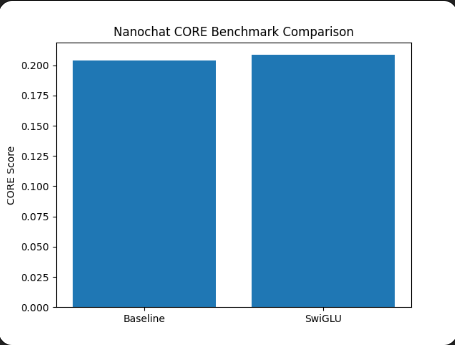
\includegraphics[width=0.55\linewidth]{p4/Screenshot 2026-03-06 113232.png}
\caption{Aggregate CORE scores.}
\label{fig:part4_core_bar}
\end{figure}

\begin{figure}[H]
\centering
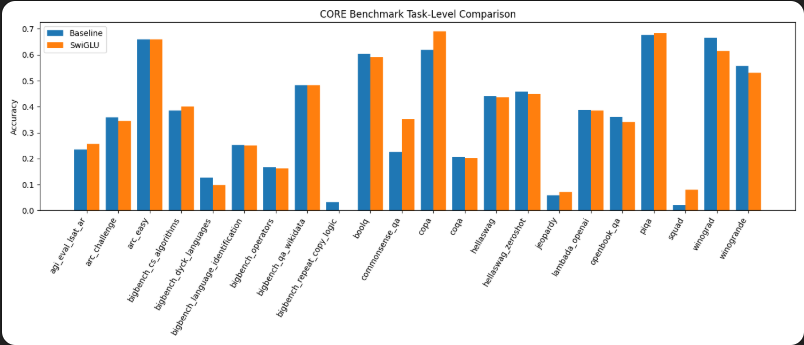
\includegraphics[width=\linewidth]{p4/Screenshot 2026-03-06 121848.png}
\caption{Per-task CORE benchmark scores for the baseline and SwiGLU nanochat models.}
\label{fig:part4_core_tasks}
\end{figure}

Task-level results are shown in Table~\ref{tab:part4_task_level_results}.

\begin{table}[H]
\centering
\small
\begin{tabular}{lcc}
\hline
\textbf{Benchmark} & \textbf{Baseline} & \textbf{SwiGLU} \\
\hline
agi\_eval\_lsat\_ar & 0.2348 & \textbf{0.2565} \\
arc\_challenge & \textbf{0.3584} & 0.3456 \\
arc\_easy & 0.6599 & 0.6599 \\
bigbench\_cs\_algorithms & 0.3841 & \textbf{0.4008} \\
bigbench\_dyck\_languages & \textbf{0.1260} & 0.0990 \\
bigbench\_language\_identification & \textbf{0.2520} & 0.2510 \\
bigbench\_operators & \textbf{0.1667} & 0.1619 \\
bigbench\_qa\_wikidata & 0.4816 & \textbf{0.4818} \\
bigbench\_repeat\_copy\_logic & \textbf{0.0312} & 0.0000 \\
boolq & \textbf{0.6043} & 0.5914 \\
commonsense\_qa & 0.2260 & \textbf{0.3522} \\
copa & 0.6200 & \textbf{0.6900} \\
coqa & \textbf{0.2068} & 0.2026 \\
hellaswag & \textbf{0.4409} & 0.4359 \\
hellaswag\_zeroshot & \textbf{0.4573} & 0.4489 \\
jeopardy & 0.0586 & \textbf{0.0709} \\
lambada\_openai & \textbf{0.3868} & 0.3842 \\
openbook\_qa & \textbf{0.3600} & 0.3420 \\
piqa & 0.6763 & \textbf{0.6823} \\
squad & 0.0219 & \textbf{0.0799} \\
winograd & \textbf{0.6667} & 0.6154 \\
winogrande & \textbf{0.5564} & 0.5304 \\
\hline
\end{tabular}
\caption{Task-level CORE benchmark results.}
\label{tab:part4_task_level_results}
\end{table}

The baseline performs slightly better on tasks resembling language
modeling and narrative completion (e.g., HellaSwag, BoolQ). In contrast,
SwiGLU improves several reasoning-oriented tasks such as
\texttt{commonsense\_qa}, \texttt{copa}, and \texttt{squad}. This suggests
that gated MLP layers may influence internal representations used in
reasoning tasks.

\subsubsection{Training Dynamics}

\begin{figure}[H]
\centering

\begin{minipage}{0.9\linewidth}
\centering
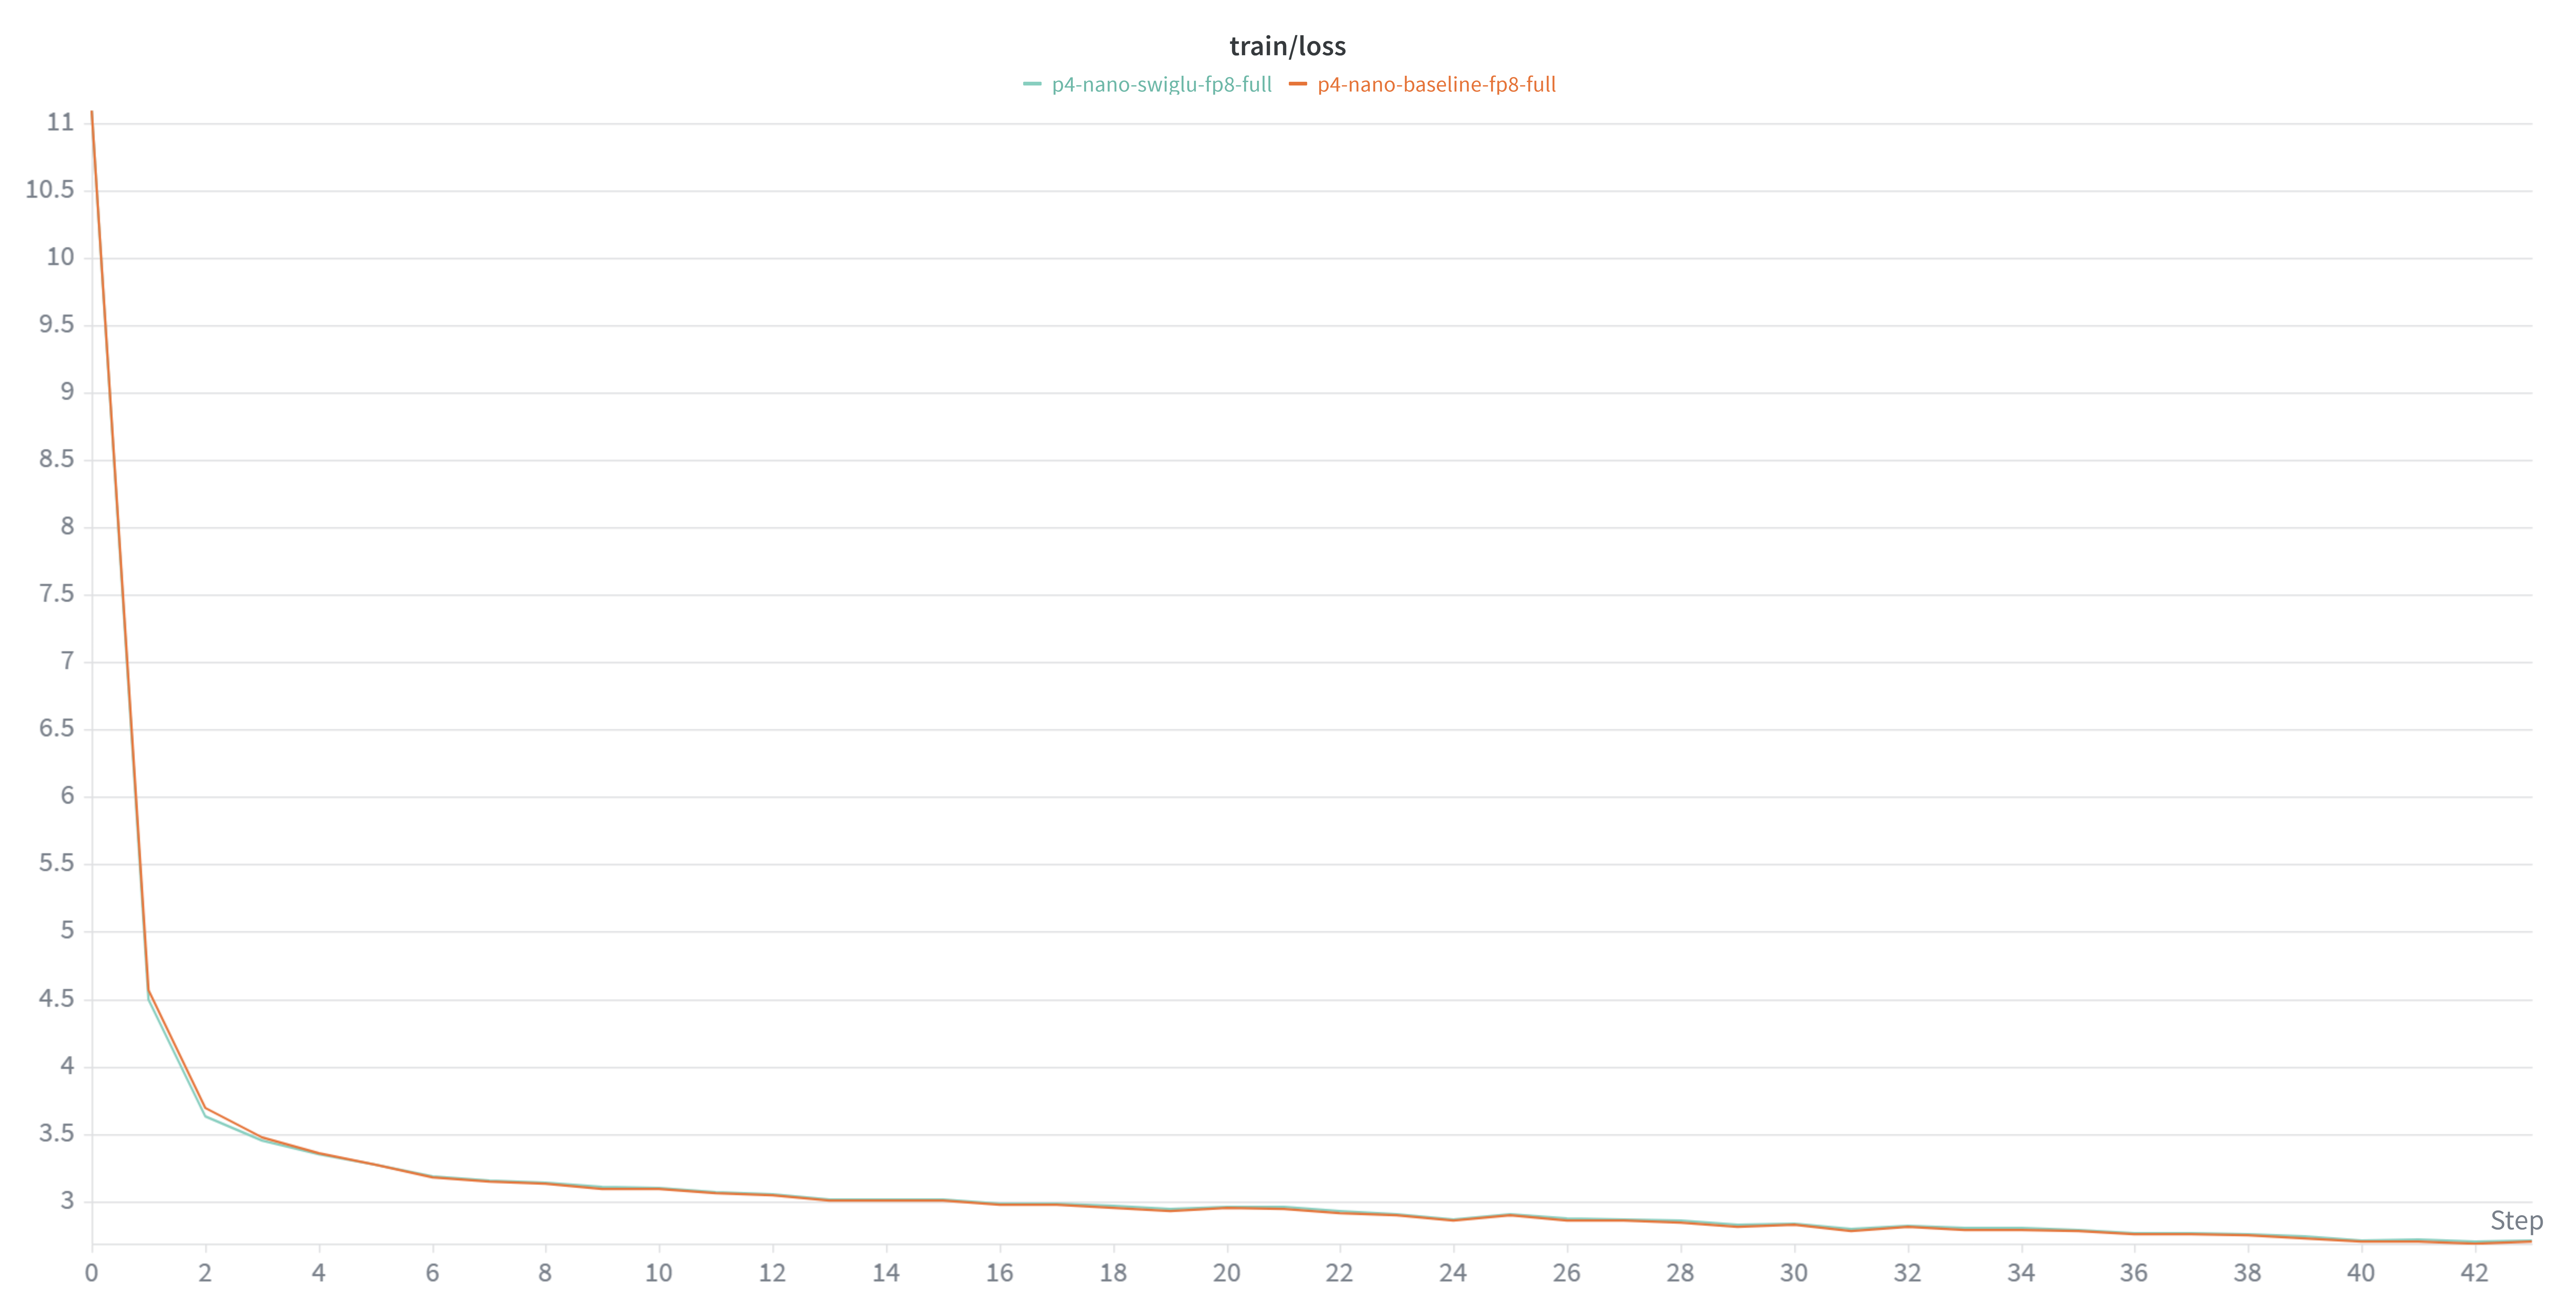
\includegraphics[width=\linewidth]{p4/W&B Chart 3_6_2026, 11_33_18 AM.png}
\subcaption{Training Loss}
\end{minipage}

\vspace{0.6em}

\begin{minipage}{0.48\linewidth}
\centering
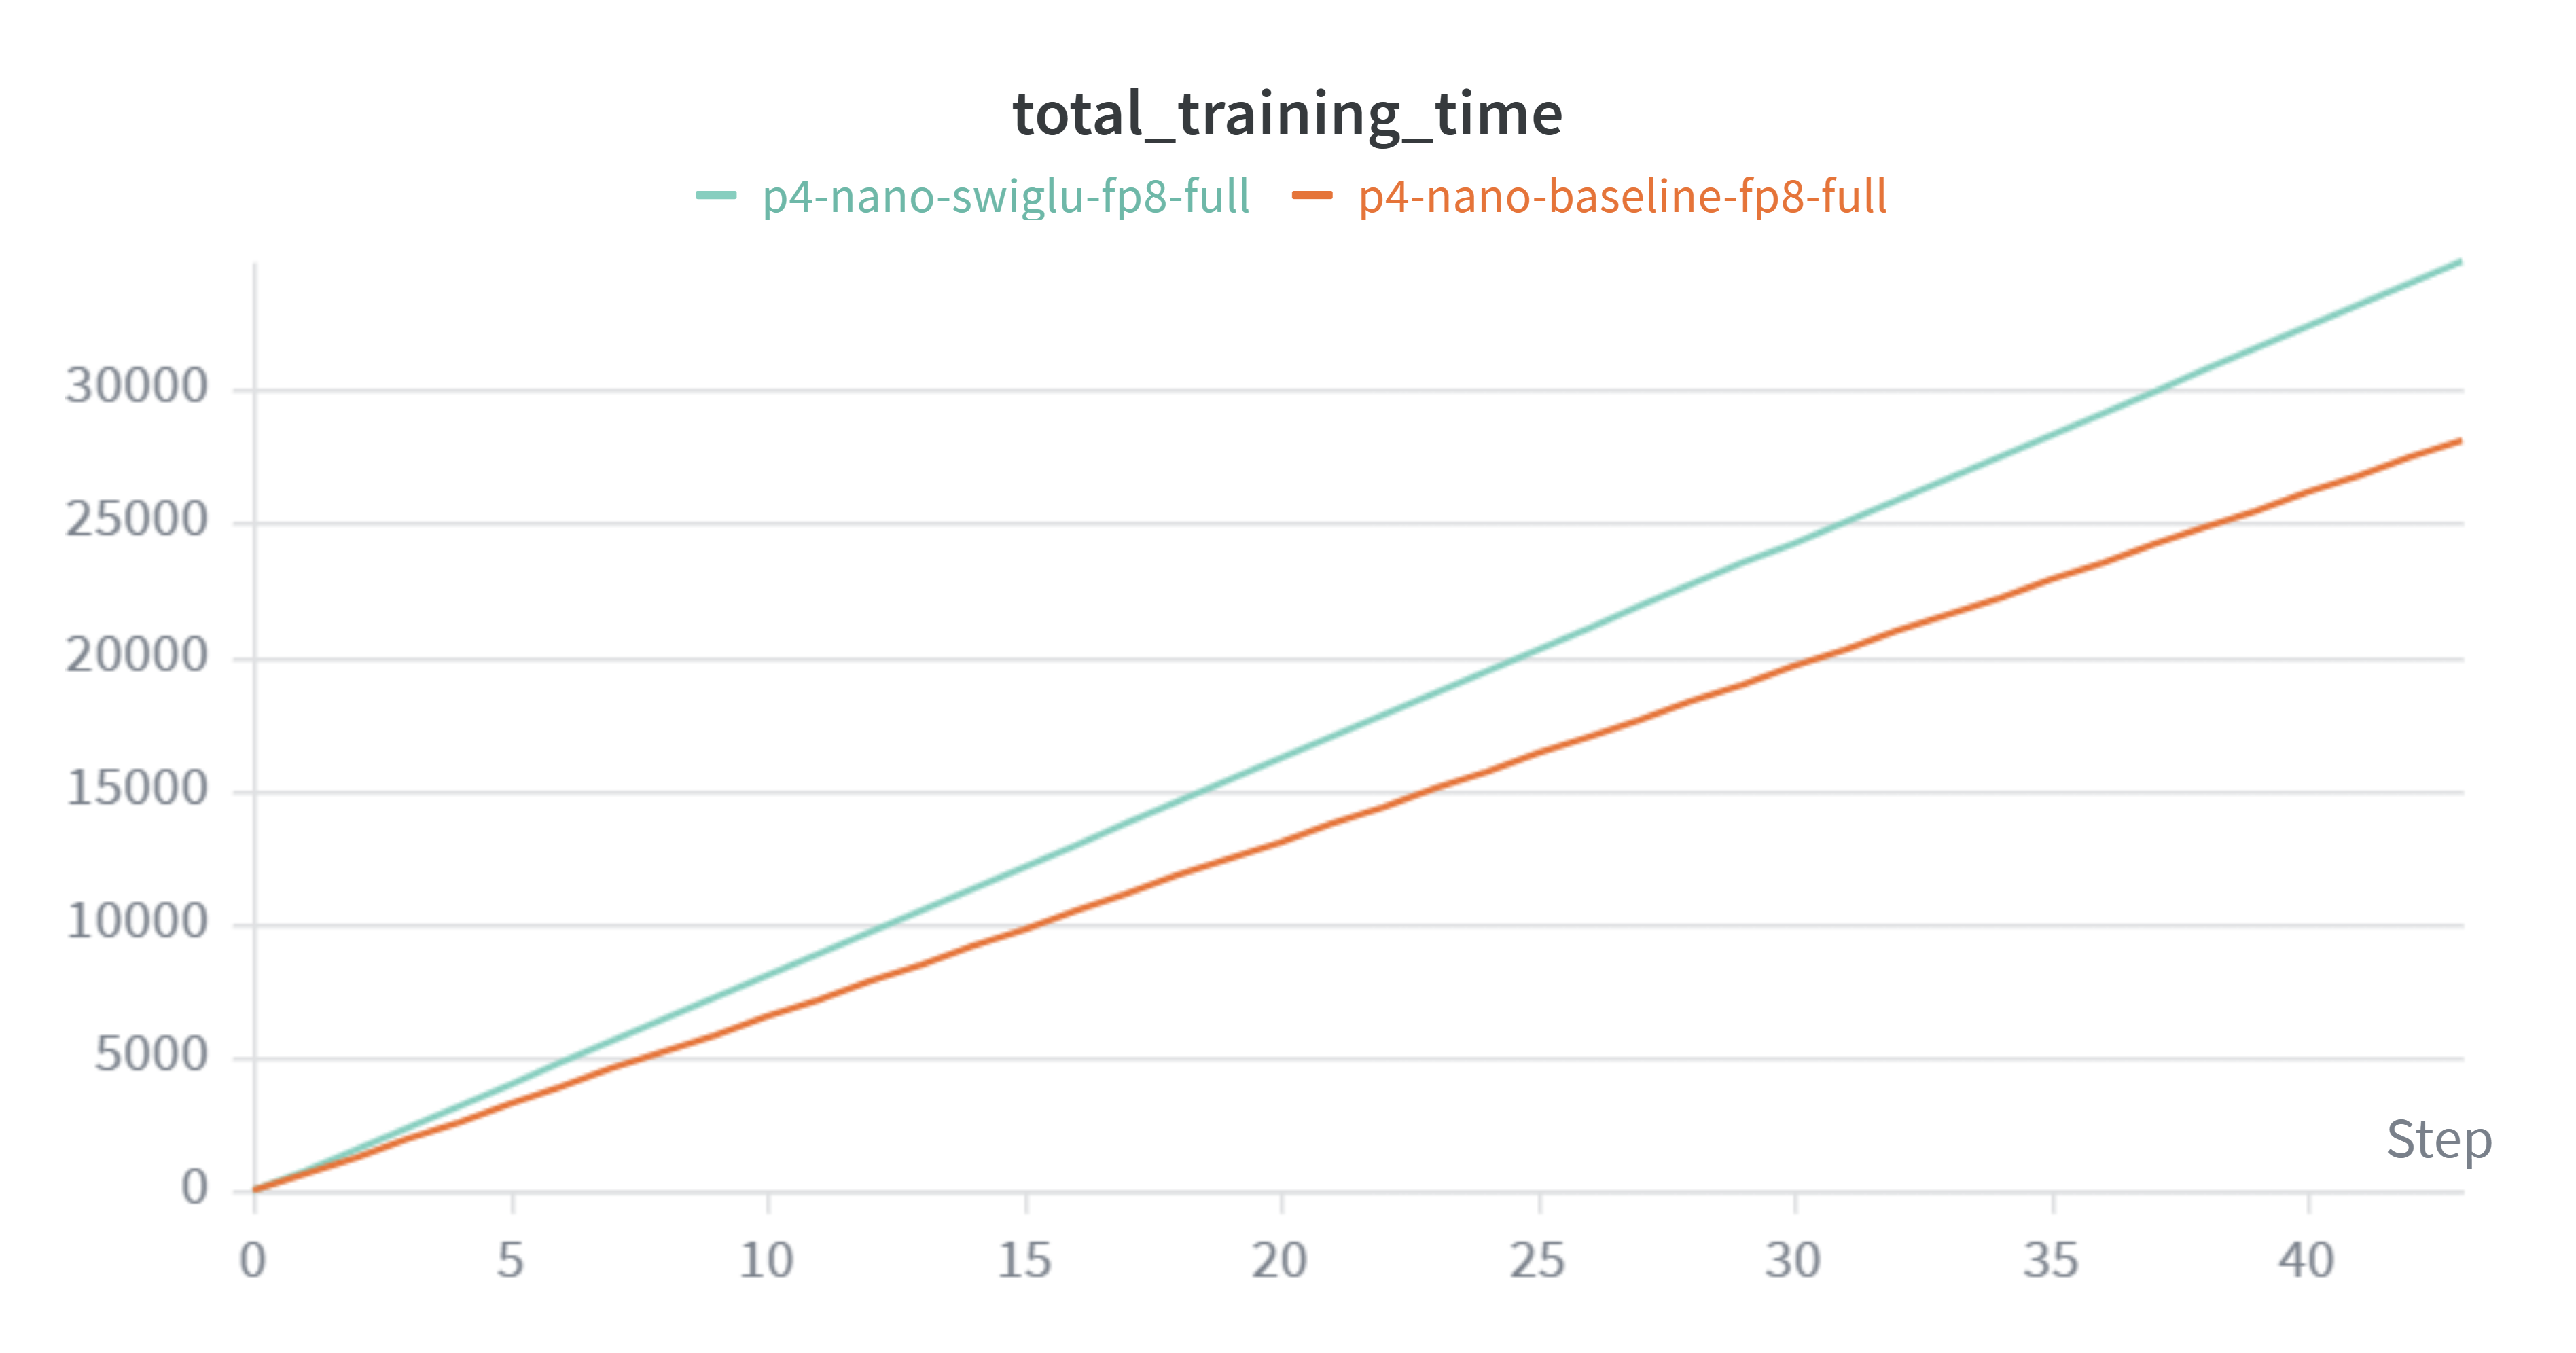
\includegraphics[width=\linewidth]{p4/W&B Chart 3_6_2026, 11_51_35 AM.png}
\subcaption{Training Time}
\end{minipage}
\hfill
\begin{minipage}{0.48\linewidth}
\centering
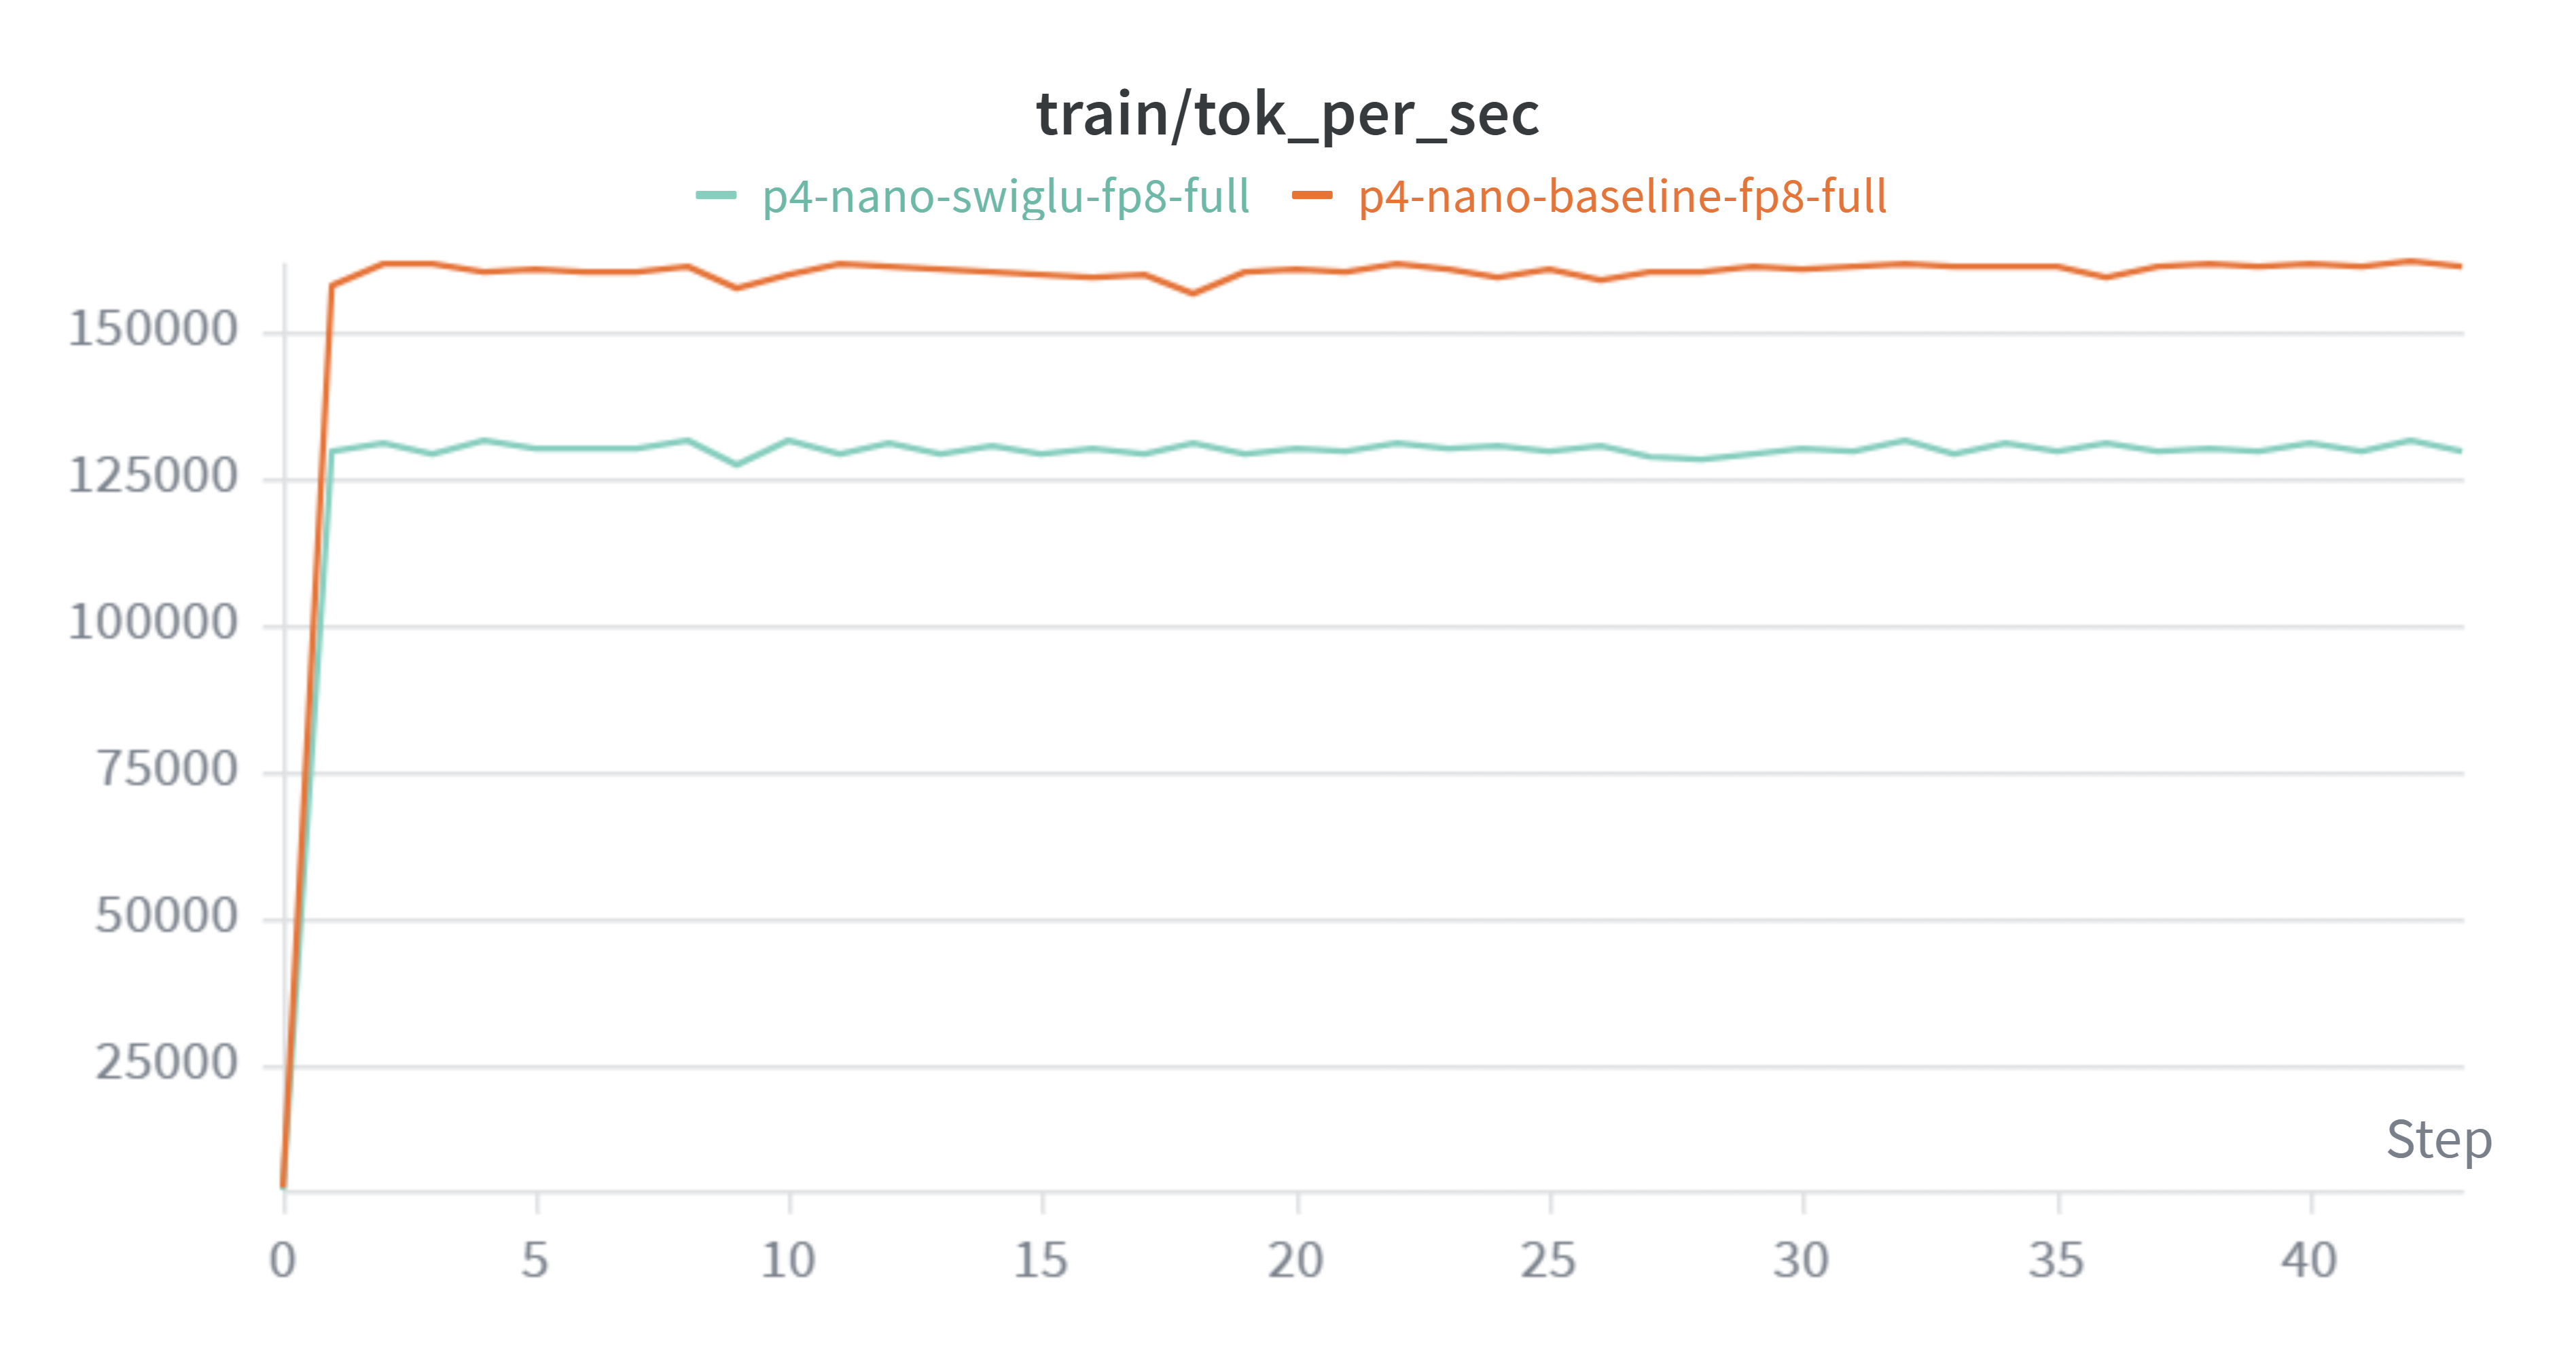
\includegraphics[width=\linewidth]{p4/W&B Chart 3_6_2026, 11_51_43 AM.png}
\subcaption{Token Throughput}
\end{minipage}

\caption{Training dynamics comparison between nanochat models.}
\label{fig:training_dynamics}

\end{figure}

Both models exhibit nearly identical loss curves, indicating similar
optimization behavior. However, the baseline maintains higher token
throughput ($\sim160$k tokens/sec) compared to the SwiGLU model
($\sim130$k tokens/sec), resulting in shorter training time.

This difference is also reflected in compute cost. The baseline training
required approximately \$33.80 in Modal compute credits, while the
SwiGLU experiment required \$44.12.

\subsubsection{Comparison with Picochat}

At the pico scale, the baseline architecture outperformed all variants
under both BPB and CORE:

\begin{itemize}
\item Pico baseline: BPB 1.0575, CORE 0.0615
\item Pico SwiGLU: BPB 1.0589, CORE 0.0554
\end{itemize}

At the nano scale, the baseline still achieves better BPB but SwiGLU
slightly surpasses it in CORE. This demonstrates that architectural
effects can change with model scale. While the modification does not
dominate overall, it becomes more competitive as model capacity
increases.

\subsection{Emergent Abilities}

Emergent abilities refer to capabilities that appear in larger models
but are absent or unreliable in smaller ones. To investigate this
phenomenon, we tested both picochat and nanochat models on a set of
diagnostic questions covering factual knowledge, scientific explanation,
and logical reasoning.

We selected questions where nanochat produced meaningful answers while
picochat failed or generated nonsensical output. See Table~\ref{tab:emergent_questions} for the list of questions.

\begin{table}[H]
\centering
\small
\begin{tabular}{p{0.95\linewidth}}
\hline
\textbf{Emergent Ability Questions} \\
\hline
1. What is the capital city of Australia? \\
2. Which country has the city of Barcelona? \\
3. Who wrote the novel \textit{1984}? \\
4. What is the largest ocean on Earth? \\
5. What gas do humans breathe in that plants produce during photosynthesis? \\
6. Why does the sky appear blue during the day? \\
7. Why do objects fall toward the ground on Earth? \\
8. What part of a plant performs photosynthesis? \\
9. What happens to water when it freezes? \\
10. If all cats are animals and all animals breathe air, do cats breathe air? \\
\hline
\end{tabular}
\caption{Questions demonstrating emergent abilities when scaling from
picochat to nanochat.}
\label{tab:emergent_questions}
\end{table}


The picochat model frequently produced incoherent or repetitive
responses. In contrast, both nanochat models correctly answered several
questions, identifying facts such as \textit{Canberra} as Australia's
capital and \textit{oxygen} as the gas produced during photosynthesis.

Between the two nanochat variants, qualitative differences were small.
The baseline model tended to produce longer explanations, whereas the
SwiGLU model often produced shorter and more direct answers.

Overall, these examples illustrate that scaling from picochat to
nanochat enables the model to retrieve factual knowledge and generate
basic explanations that are largely absent in the smaller model.

\subsection{Discussion}

Overall, three conclusions emerge from the experiments.

First, scaling the model from picochat to nanochat substantially improves
language modeling quality and benchmark performance.

Second, the SwiGLU architecture slightly improves several reasoning
benchmarks but does not outperform the baseline in BPB and incurs
additional computational cost.

Third, architectural modifications can behave differently at different
scales, highlighting the importance of empirical evaluation when
designing transformer architectures.

\subsection{Codebase Organization}

This project consists of two main codebases: the modified \texttt{nanochat}
training framework used for model development and evaluation, and the
\texttt{AI-Accountant} repository that organizes the experimental workflow
for Assignment~3. The following section summarizes the key modifications and
directory structure used to support the experiments.

\subsubsection{Nanochat Modifications}

The nanochat framework was extended to support architectural ablations and
more robust evaluation. Compared to the original upstream repository, three
files were modified.

\begin{itemize}

\item \textbf{\texttt{nanochat/gpt.py}} \\
This file contains the core transformer architecture implementation.
Several extensions were introduced to support the architectural ablations
explored in this assignment. Specifically, the model now supports multiple
MLP variants (\texttt{relu2} and \texttt{swiglu}), optional residual
scaling through a LayerScale variant, and a configurable
\texttt{layerscale\_init} parameter controlling residual scaling strength.
Additionally, dynamic rotary embedding cache growth was implemented through
the \texttt{\_ensure\_rotary\_cache} function to allow evaluation with longer
sequence lengths than those used during training.

\item \textbf{\texttt{scripts/base\_train.py}} \\
The training entrypoint was modified to expose the new architectural
configuration options through the command-line interface and configuration
files. This allows experiments to select between the baseline ReLU$^2$ MLP,
SwiGLU MLP, and residual variants directly through experiment YAML files
without modifying the model implementation.

\item \textbf{\texttt{scripts/base\_eval.py}} \\
The evaluation pipeline was extended to support resumable CORE benchmark
evaluation. Progress files are written under a \texttt{base\_eval\_progress}
directory, enabling interrupted evaluation runs to resume without repeating
completed tasks. Additional features include task-level progress tracking,
support for \texttt{max-per-task} evaluation limits, and progress-path
reporting in logs for easier monitoring of long-running benchmark jobs.

\end{itemize}

These modifications enable flexible experimentation with architectural
variants while ensuring that long-running evaluation jobs can be resumed
safely.

\subsubsection{Assignment Repository Structure}


\definecolor{dircmt}{HTML}{6A737D}
\definecolor{filecmt}{HTML}{FF9966}
\newcommand{\cmt}[1]{\normalfont{\textcolor{dircmt}{\textit{#1}}}}
\newcommand{\fcmt}[1]{\normalfont{\textcolor{filecmt}{\textit{#1}}}}

How the \texttt{a3/} folder is organized inside the AI-Accountant repo is explained. The
structure follows the assignment's four-part layout.

\subsection*{Layout}

\begin{forest}
  for tree={
    font=\ttfamily,
    grow'=0,
    child anchor=west,
    parent anchor=south,
    anchor=west,
    calign=first,
    edge path={
      \noexpand\path [draw, -{|}] (!u.south west) +(7.5pt,0) |- node[fill,inner sep=1.25pt] {} (.child anchor)\forestoption{edge label};
    },
    before typesetting nodes={
      if n=1 {insert before={[,phantom]}} {}
    },
    fit=band,
    before computing xy={l=19.5pt},
    s sep=4pt,
  }
  [a3/
    [docs/ \cmt{teammate onboarding and shared references}]
    [shared/ \cmt{pipeline infrastructure used by all parts}
      [configs/ \cmt{smoke-test YAMLs for pipeline validation}]
      [scripts/ \cmt{Modal pipeline code}
        [main.py \fcmt{local entrypoint: reads YAML config, launches Modal run}]
        [shared/
          [infra.py \fcmt{Modal app, image, volume, and secrets definitions}]
          [helpers.py \fcmt{pure utilities: git checkout, checkpoint discovery, eval parsing}]
        ]
        [runners/
          [run.py \fcmt{orchestrator: dispatches training stages and evals in parallel}]
          [train.py \fcmt{runs nanochat training on a Modal GPU}]
          [evaluate.py \fcmt{runs BPB, CORE, and custom evals on a Modal GPU}]
        ]
      ]
    ]
    [p2/ \cmt{picochat ablation}
      [configs/
        [p2\_baseline.yaml \fcmt{vanilla picochat baseline}]
        [p2\_swiglu.yaml \fcmt{SwiGLU activation ablation}]
        [p2\_layerscale.yaml \fcmt{LayerScale ablation}]
        [p2\_swiglu\_layerscale.yaml \fcmt{combined SwiGLU + LayerScale ablation}]
        [p2\_*\_eval\_bpb\_core.yaml \fcmt{eval-only configs for each ablation}]
        [p2\_swiglu\_layerscale\_smoke.yaml \fcmt{quick smoke test for combined variant}]
      ]
      [training-troubleshooting.md \fcmt{notes on training issues encountered}]
    ]
    [p3/ \cmt{continued on next page}]
    [p4/ \cmt{continued on next page}]
  ]
\end{forest}

\newpage

\subsection*{Layout (continued)}

\begin{forest}
  for tree={
    font=\ttfamily,
    grow'=0,
    child anchor=west,
    parent anchor=south,
    anchor=west,
    calign=first,
    edge path={
      \noexpand\path [draw, -{|}] (!u.south west) +(7.5pt,0) |- node[fill,inner sep=1.25pt] {} (.child anchor)\forestoption{edge label};
    },
    before typesetting nodes={
      if n=1 {insert before={[,phantom]}} {}
    },
    fit=band,
    before computing xy={l=19.5pt},
    s sep=4pt,
  }
  [a3/
    [p3/ \cmt{context window extension}
      [docs/ \cmt{literature review, training config, eval design, final spec}]
      [configs/
        [p3\_baseline.yaml \fcmt{three-stage context extension experiment}]
        [p3\_eval\_only.yaml \fcmt{re-run evals on existing checkpoints}]
        [p3\_core\_evals.yaml \fcmt{CORE-only eval variant}]
        [p3\_from\_p2\_template.yaml \fcmt{template to eval P2's best model on P3 evals}]
      ]
      [evals/
        [context\_length\_eval.py \fcmt{positional perplexity eval on PG19 test split}]
      ]
      [results/ \cmt{run outputs}
        [core\_csvs/ \cmt{CORE per-task accuracy CSVs}]
        [custom\_evals/ \cmt{positional perplexity JSONs}]
        [figures/ \cmt{plots and summary tables}]
        [tex/ \cmt{compiled writeup PDF}]
      ]
      [analysis/
        [generate\_plots.py \fcmt{builds figures and tables from fetched results}]
      ]
    ]
    [p4/ \cmt{scaling laws and emergent abilities}
      [configs/
        [p4\_nano\_baseline\_fp8.yaml \fcmt{nanochat baseline with FP8 training}]
        [p4\_nano\_swiglu\_fp8.yaml \fcmt{nanochat SwiGLU variant with FP8 training}]
        [p4\_pipeline\_smoke\_20min.yaml \fcmt{quick smoke test for nano-scale runs}]
        [p4\_*\_eval\_only.yaml \fcmt{eval-only configs for each nano model}]
        [p4\_template.yaml \fcmt{template YAML for scaling runs}]
      ]
      [scripts/
        [compare\_emergent\_abilities.py \fcmt{finds questions nanochat answers but picochat cannot}]
      ]
      [results/ \cmt{run outputs}
        [final/ \cmt{final eval CSVs and JSONs per model}]
      ]
      [emergent\_abilities\_results.txt \fcmt{emergent abilities comparison output}]
    ]
  ]
\end{forest}


\newpage
\paragraph{Part 1: Infrastructure and Orchestration}

The infrastructure and orchestration layer is implemented under
\texttt{a3/shared}. This directory contains reusable pipeline components
used by all experiments.

Key files include:

\begin{itemize}

\item \textbf{\texttt{scripts/main.py}} \\
Primary local entrypoint for running experiments from YAML configuration
files.

\item \textbf{\texttt{scripts/runners/run.py}} \\
Orchestrates the full training and evaluation pipeline by coordinating
individual stages.

\item \textbf{\texttt{scripts/runners/train.py}} \\
Implements the training worker responsible for launching model training
jobs.

\item \textbf{\texttt{scripts/runners/evaluate.py}} \\
Handles evaluation runs, including CORE benchmark execution.

\item \textbf{\texttt{scripts/shared/infra.py}} \\
Defines the Modal infrastructure configuration, including container
images, persistent volumes, and secret management.

\item \textbf{\texttt{scripts/shared/helpers.py}} \\
Provides helper utilities for parsing configuration files and managing
pipeline stages.

\end{itemize}

The \texttt{a3/docs} directory contains supporting documentation for the
infrastructure design, including interface definitions and experiment
workflow descriptions.

\paragraph{Part 2: Picochat Ablation Experiments}

All pico-scale ablation experiments are defined in
\texttt{a3/p2/configs}. These configuration files specify experiment
variants including:

\begin{itemize}
\item baseline architecture
\item SwiGLU MLP variant
\item LayerScale residual variant
\item combined architectural modifications
\item smoke-test and evaluation-only configurations
\end{itemize}

The file \texttt{training-troubleshooting.md} documents issues encountered
during early training runs and the steps taken to resume interrupted
experiments.

\paragraph{Part 3: Analysis Structure}

The \texttt{a3/p3} directory provides the structure for analysis artifacts,
including placeholders for evaluation results, documentation, and
experiment outputs. While this directory contains minimal code, it
establishes the standardized layout used for subsequent parts of the
assignment.

\paragraph{Part 4: Nanochat Experiments}

The final nanochat experiments are organized under \texttt{a3/p4}.

\begin{itemize}

\item \textbf{\texttt{configs}} \\
Contains YAML configurations for full nanochat training runs, evaluation-only
jobs, hyperparameter sweeps, and smoke-test pipelines.

\item \textbf{\texttt{results}} \\
Stores downloaded evaluation artifacts including BPB measurements,
CORE benchmark outputs, and aggregated CSV/JSON summaries used in the
analysis.

\item \textbf{\texttt{scripts/compare\_emergent\_abilities.py}} \\
A diagnostic script that generates side-by-side responses from picochat
and nanochat models to compare qualitative reasoning abilities.

\item \textbf{\texttt{emergent\_abilities\_results.txt}} \\
A generated file containing the qualitative comparison outputs used in
the emergent ability analysis in Part~4.

\end{itemize}

Overall, this structure separates reusable infrastructure code, experiment
configuration files, and analysis artifacts. This organization improves
reproducibility and makes it easier to track experimental results across
different parts of the assignment.

\input{component/part5}

% Appendix: Infrastructure and Pipeline

%% ============================================================
\appendix
\section{Infrastructure and Pipeline}
\label{sec:appendix-pipeline}
%% ============================================================

%% ============================================================
\subsection{Infrastructure Choices}
%% ============================================================

\subsubsection{Modal --- GPU Compute}

A3 needs single-GPU training jobs. Modal is the simplest platform for this: write a Python function, pick a GPU, run it. We had \$500 in academic credits, per-second billing, and Volumes (persistent networked disks) to save checkpoints between runs.

\paragraph{Why not others}
Anyscale (\$1{,}000) is built around Ray for distributed workloads---more setup than needed for single-GPU jobs. AWS (\$500) has the most overhead (EC2, SSH, drivers, storage). Snowflake (\$400 trial) is a data warehouse, not a training platform.

\paragraph{GPU selection}
Nanochat requires BF16, so A10G is the minimum. A100/H100 are faster and often cheaper in total cost due to shorter wall time.

\begin{table}[H]
\centering\small
\begin{tabular}{@{}llrr@{}}
\toprule
Part & GPU & Est.\ Time & Est.\ Cost \\
\midrule
P2 (4 ablation runs) & A100 & 1--5 hrs & \$3--13 \\
P3 (2 training stages + eval) & A100 & 1--3 hrs & \$3--8 \\
P4 (full nanochat) & H100 & 6--20 hrs & \$24--79 \\
\bottomrule
\end{tabular}
\caption{Estimated GPU time and cost per assignment part.}
\end{table}

\subsubsection{Weights \& Biases --- Experiment Tracking}

Dashboard for training curves, loss values, and run configs. Already built into nanochat---no extra code needed.

\begin{itemize}[nosep]
  \item \textbf{Project}: \texttt{490-autobook-a3} (shared across all parts)
  \item \textbf{Namespacing}: each run tagged \texttt{p2}, \texttt{p3}, or \texttt{p4}
  \item \textbf{Reproducibility}: every run logs which nanochat commit it used
\end{itemize}

\subsubsection{YAML Configs --- Run Specification}

Each experiment is a YAML file whose fields map directly to nanochat's command-line flags (\texttt{--depth}, \texttt{--max-seq-len}, etc.). The \texttt{nanochat\_ref} field picks which fork branch or tag to run. No extra config framework needed---nanochat already parses its own arguments.

%% ============================================================
\subsection{Pipeline Architecture}
%% ============================================================

The pipeline reads a YAML config, sends training and evaluation jobs to Modal GPUs, and writes results to a Modal Volume and W\&B. All experiments are controlled via config---no pipeline code changes needed between runs.

\subsubsection{Code Structure}

\begin{forest}
  for tree={
    font=\ttfamily\small,
    grow'=0,
    child anchor=west,
    parent anchor=south,
    anchor=west,
    calign=first,
    edge path={
      \noexpand\path [draw, -{|}] (!u.south west) +(7.5pt,0) |- node[fill,inner sep=1.25pt] {} (.child anchor)\forestoption{edge label};
    },
    before typesetting nodes={
      if n=1 {insert before={[,phantom]}} {}
    },
    fit=band,
    before computing xy={l=15pt},
    s sep=4pt,
  }
  [a3/shared/scripts/
    [main.py \normalfont{\textit{--- parses YAML, calls} \texttt{run.remote()}}]
    [shared/
      [infra.py \normalfont{\textit{--- app, image, volume, secrets, setup()}}]
      [helpers.py \normalfont{\textit{--- pure Python utilities}}]
    ]
    [runners/
      [run.py \normalfont{\textit{--- orchestrator: spawns stages then evals}}]
      [train.py \normalfont{\textit{--- one training stage per GPU}}]
      [evaluate.py \normalfont{\textit{--- one checkpoint eval per GPU}}]
    ]
  ]
\end{forest}

\subsubsection{Execution Flow}

\begin{figure}[H]
\centering
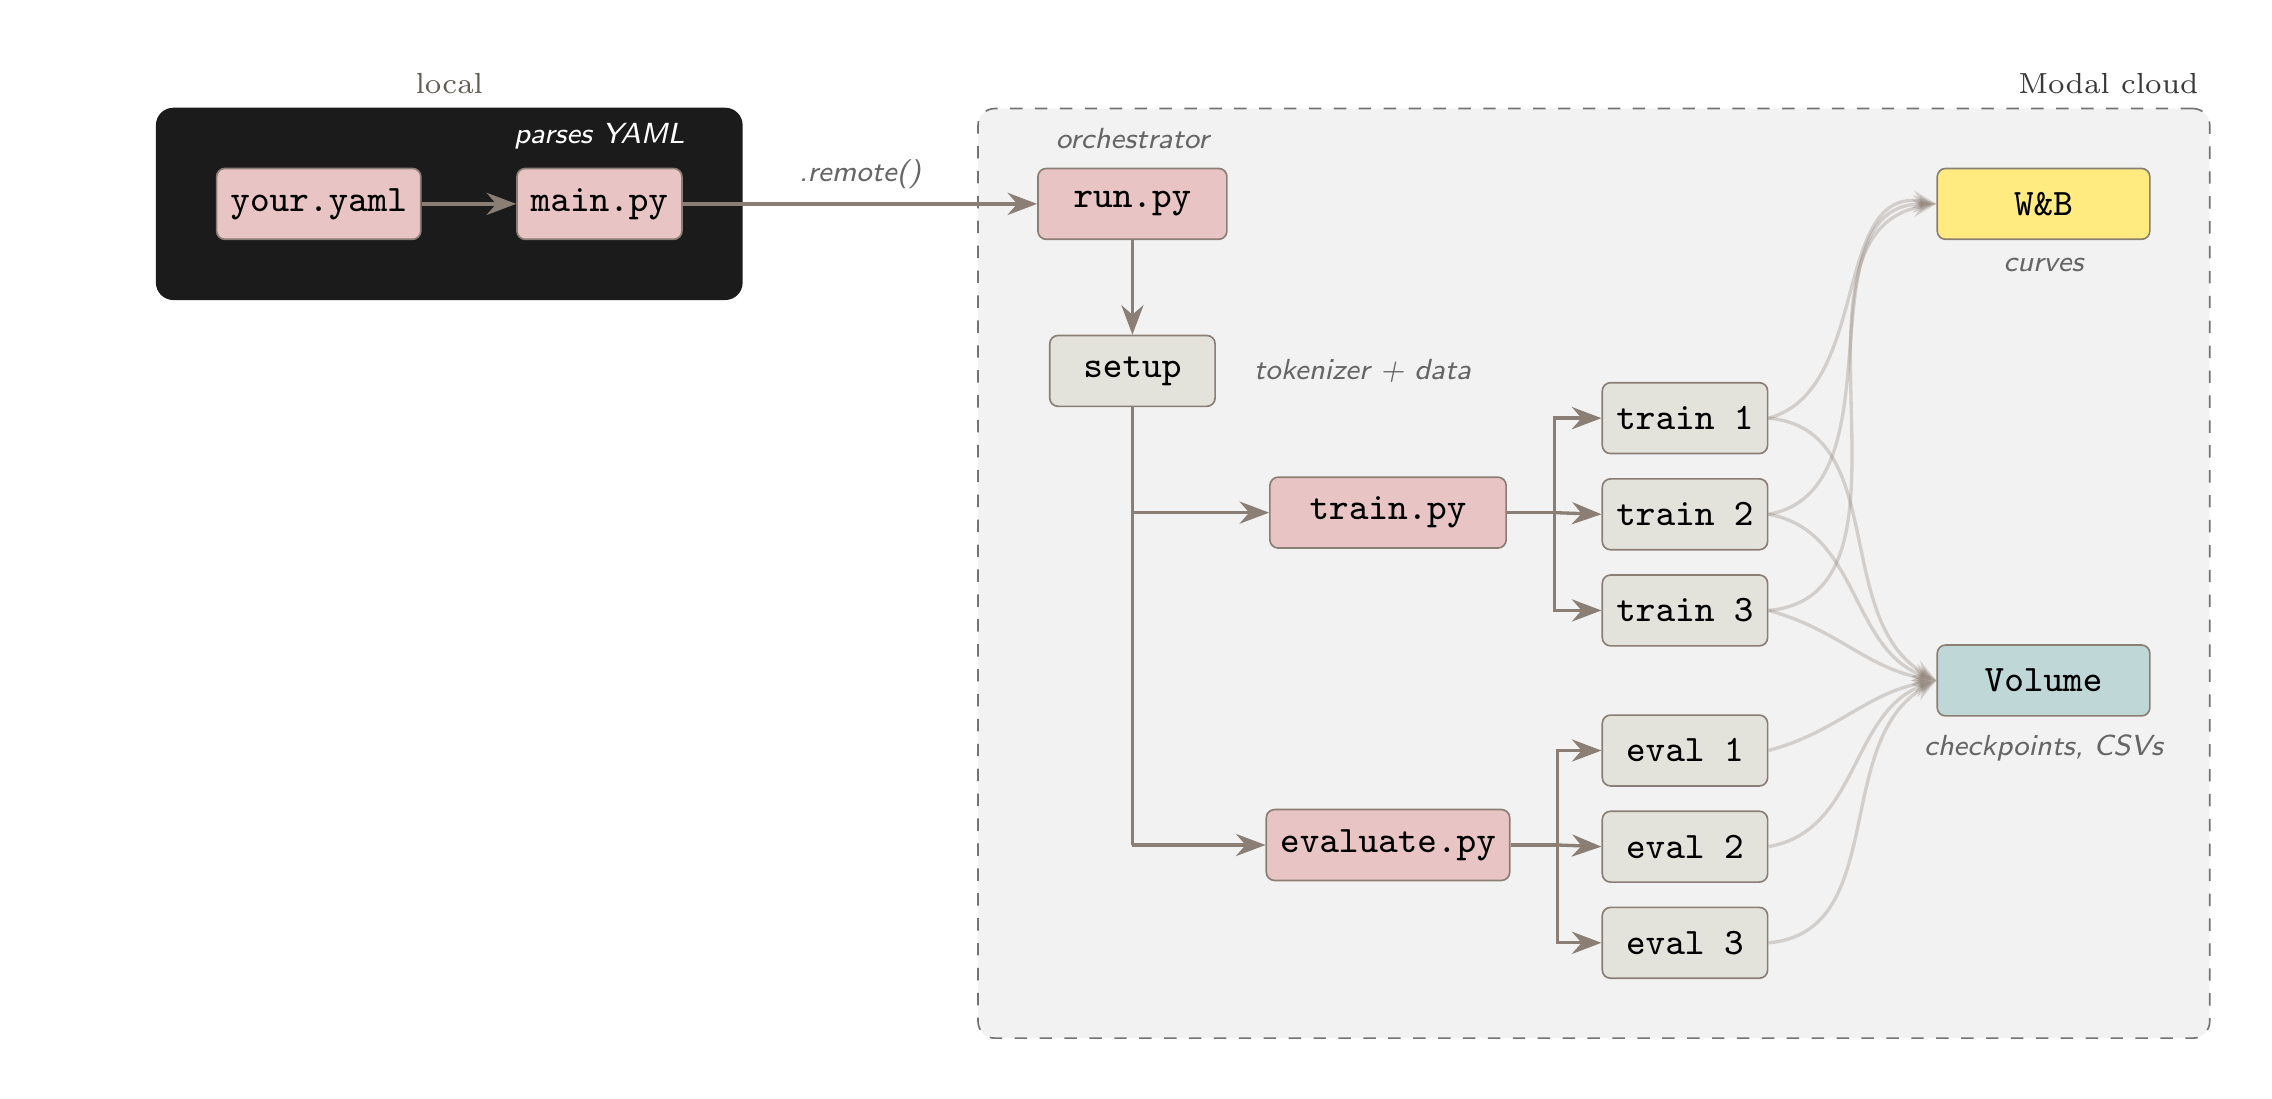
\includegraphics[width=\linewidth]{pipeline_diagram.png}
\caption{Pipeline architecture. A YAML config is parsed locally, then dispatched to Modal cloud for training and evaluation. Training stages write checkpoints to a persistent Volume and metrics to W\&B; evaluations read checkpoints from the Volume and write results back.}
\label{fig:pipeline}
\end{figure}

The workflow is two steps: (1)~write a YAML config specifying model depth, sequence length, GPU type, and which evals to run, then (2)~run a single command:

\begin{lstlisting}
modal run --detach a3/shared/scripts/main.py \
    --config a3/<part>/configs/<your-config>.yaml
\end{lstlisting}

Modal spins up GPU containers, trains the model, runs evals, and writes results to a Modal Volume (checkpoints, CSVs, JSONs) and W\&B (training curves). The \texttt{--detach} flag keeps the pipeline running on Modal independent of the local terminal.

\subsubsection{Nanochat Fork}

We maintain a fork of Karpathy's nanochat at \url{https://github.com/seonghyunban/nanochat} so that teammates can modify the architecture without touching the original code. The pipeline integrates the fork as follows:

\begin{enumerate}[nosep]
  \item The Modal container image clones the fork once at build time and caches it.
  \item Before every run, the container does \texttt{git fetch} then checks out whichever branch or tag the YAML config's \texttt{nanochat\_ref} field specifies.
  \item No container rebuild is needed when new code is pushed---the next run picks it up automatically.
\end{enumerate}

\paragraph{Branch strategy}

\begin{itemize}[nosep]
  \item \texttt{master} --- original nanochat, frozen. All baseline runs use this.
  \item \texttt{p2} --- P2's architecture modifications (SwiGLU, LayerScale), branched from \texttt{master}.
  \item \texttt{p3-log-every} --- P3's fork patch adding a \texttt{--log-every} flag for finer W\&B logging.
  \item \texttt{baseline-v0} --- immutable tag on \texttt{master}. Safety net: even if someone pushes to \texttt{master}, this tag never moves.
\end{itemize}


\end{document}
